\documentclass[11pt,letterpaper]{article}

\usepackage[english]{babel}
\usepackage[utf8]{inputenc}
\usepackage[T1]{fontenc}
\usepackage{lmodern}
\usepackage{amsmath,amssymb,mathtools}
\usepackage{amsthm}
\usepackage{physics}
\usepackage{geometry}
\usepackage{enumitem}
\usepackage{needspace}
\usepackage{tikz}
\usepackage{pgfplots}
\pgfplotsset{compat=1.18}
\definecolor{diagramblue}{RGB}{0,142,190}
\definecolor{diagramgreen}{RGB}{67,150,45}
\definecolor{diagramred}{RGB}{210,40,30}
\usetikzlibrary{arrows.meta,calc,positioning}
\usepackage{hyperref}

\hypersetup{
  pdftitle={Lambda phi4 theory and Feynman rules in position space},
  pdfauthor={Omar Corona Tejeda},
  colorlinks=true,
  linkcolor=blue,
  urlcolor=blue,
  citecolor=blue
}

\geometry{margin=2.2cm}
\setlength{\parindent}{0pt}
\setlength{\parskip}{0.45em}
\interfootnotelinepenalty=10000
\raggedbottom
\clubpenalty=10000
\widowpenalty=10000
\setlist[itemize]{leftmargin=1.3em}

\theoremstyle{definition}
\newtheorem{definicion}{Definition}
\theoremstyle{definition}
\newtheorem{observacion}{Remark}
\newtheorem{ejemplo}{Example}
\AddToHook{env/ejemplo/begin}{\pushQED{\qed}}
\AddToHook{env/ejemplo/end}{\par\nobreak\vspace{0.35em}\noindent\popQED}
\newcommand{\eqbox}[1]{\boxed{\displaystyle #1}}
\newcounter{footnotequation}
\newcommand{\fnEqTag}{\refstepcounter{footnotequation}\tag{\Roman{footnotequation}}}
\newcounter{diagrama}
\newcommand{\diagramcaption}[1]{%
  \refstepcounter{diagrama}%
  \par\vspace{0.7em}{\footnotesize\textbf{Figure \thediagrama.} #1}\par\vspace{0.4em}%
}
\newcommand{\qftFreeDiagram}{%
  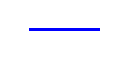
\begin{tikzpicture}[baseline=-0.5ex,scale=0.45]
    \draw[blue,very thick] (-1,0)--(1,0);
  \end{tikzpicture}%
}
\newcommand{\qftTadpoleDiagram}{%
  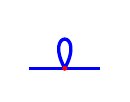
\begin{tikzpicture}[baseline=-0.5ex,scale=0.45]
    \draw[blue,very thick] (-1,0)--(1,0);
    \draw[blue,very thick] (0,0)
      .. controls (-0.6,1.1) and (0.6,1.1) .. (0,0);
    \fill[red] (0,0) circle (2pt);
  \end{tikzpicture}%
}
\newcommand{\qftVacuumDiagram}{%
  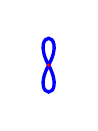
\begin{tikzpicture}[baseline=-0.5ex,scale=0.35]
    \draw[blue,very thick] (0,0)
      .. controls (-0.7,1.3) and (0.7,1.3) .. (0,0);
    \draw[blue,very thick] (0,0)
      .. controls (-0.7,-1.3) and (0.7,-1.3) .. (0,0);
    \fill[red] (0,0) circle (2pt);
  \end{tikzpicture}%
}
\newcommand{\qftChainDiagram}{%
  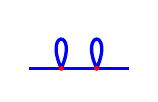
\begin{tikzpicture}[baseline=-0.5ex,scale=0.45]
    \draw[blue,very thick] (-1.4,0)--(1.4,0);
    \foreach \x in {-0.5,0.5} {
      \draw[blue,very thick] (\x,0)
        .. controls (\x-0.5,1.1) and (\x+0.5,1.1) .. (\x,0);
      \fill[red] (\x,0) circle (2pt);
    }
  \end{tikzpicture}%
}

\title{$\lambda\phi^4$ theory and Feynman rules\\
in position space}
\author{Omar Corona Tejeda\\
\href{mailto:omarct1989@ciencias.unam.mx}{omarct1989@ciencias.unam.mx}\\[0.2cm]
\href{https://artinnether.github.io/the_mathematical_physics_project/}
{The Mathematical Physics Project}}
\date{September 30, 2026}

\begin{document}

\maketitle

\begin{abstract}
The position-space Feynman rules are derived for the two-point correlator
of real scalar $\lambda\phi^4$ theory. The Schrödinger, Heisenberg, and
interaction pictures are first defined, distinguishing free evolution
from full evolution. Nested commutators and the Baker--Campbell--Hausdorff
formula are used to reconstruct the free-field mode expansion and obtain
the interaction Hamiltonian.

The Gell-Mann--Low formula, the Dyson series, and Wick's theorem translate
contractions into propagators, vertices, and spacetime integrals. The
cancellation of vacuum bubbles is explained, first-order contributions
are calculated, and the three connected second-order topologies are
presented with their integrals and symmetry factors. Figures and examples connect field evolution to operator calculations and
show how diagrammatic rules emerge from the combinatorics of contractions. Loop integrals remain formal; their regularization and
renormalization are not developed.
\end{abstract}

\section{Introduction}

The passage from quantum-field dynamics to Feynman rules requires bringing
together several structures: the evolution of states and operators, the
choice of vacuum, time ordering, and the combinatorics of contractions.
The simplicity of a diagram is the result of this work. Understanding how
it is constructed reveals what each line represents, which operation a
vertex introduces, and where the coefficient accompanying a contribution
comes from. These notes develop that construction for the two-point
correlator of real scalar $\lambda\phi^4$ theory in position space.

The first task is to identify the operators used in the calculation.
The Schrödinger, Heisenberg, and interaction pictures share initial data
but distribute time evolution differently between states and operators.
Distinguishing the free Hamiltonian from the full Hamiltonian establishes
the role of $\phi_I$ and its relation to the interacting field $\phi_H$.
Nested commutators and the Baker--Campbell--Hausdorff formula reconstruct
the mode expansion, explicitly verifying the free evolution underlying
the perturbative development and yielding the interaction Hamiltonian.

The second task is to turn this operator structure into an organized
calculation. The Gell-Mann--Low formula relates the interacting-vacuum
correlator to expectation values in the free vacuum; the Dyson series
organizes interaction insertions, and Wick's theorem reduces them to
products of propagators. We follow the contractions through the
first-order contributions and the three connected second-order topologies,
including their integrals and symmetry factors. Normalization establishes
which pieces cancel: vacuum bubbles disappear, while loops attached to
the external points remain.

The central result is a justification of the Feynman rules from the
canonical formalism and contraction counting. Once this foundation is
established, subsequent calculations can be organized through diagrams
without reconstructing the full operator expansion in each case.
We use $\hbar=c=1$, the metric $(+,-,-,-)$, and an interaction without
normal ordering, working around the symmetric vacuum. Loop integrals
remain formal; their evaluation, regularization, and renormalization
constitute the next stage of the analysis.

\section{\texorpdfstring{$\lambda\phi^4$}{lambda phi4} theory}

We consider a real scalar field in the perturbative regime around
the symmetric vacuum, with $m^2>0$ and $\lambda\geq0$. Its Lagrangian is
\begin{equation}
  \eqbox{\mathcal{L}
  \coloneqq\frac{1}{2}\partial_\mu\phi\,\partial^\mu\phi
  -\frac{m^2}{2}\phi^2
  -\frac{\lambda}{4!}\phi^4.}
\end{equation}
The dot over the field denotes its partial derivative with respect to
time, with the spatial coordinate held fixed:
\begin{equation}
  \dot\phi(t,\mathbf{x})
  \coloneqq\partial_t\phi(t,\mathbf{x})
  =\frac{\partial\phi(t,\mathbf{x})}{\partial t}
  =\partial_0\phi(t,\mathbf{x}).
\end{equation}
With the metric convention $(+,-,-,-)$, the canonical momentum conjugate to the field is
\begin{equation}
  \pi(t,\mathbf{x})
  \coloneqq\frac{\partial\mathcal L}{\partial\dot\phi(t,\mathbf{x})}
  =\dot\phi(t,\mathbf{x}).
\end{equation}
The Hamiltonian density is
\begin{equation}
  \eqbox{\mathcal{H}
  \coloneqq\frac{1}{2}\pi^2
  +\frac{1}{2}\abs{\grad\phi}^2
  +\frac{m^2}{2}\phi^2
  +\frac{\lambda}{4!}\phi^4.}
\end{equation}

Integrating the Hamiltonian density over space, we separate the free part
from the interaction:
\begin{equation}
  \boxed{\begin{aligned}
  H(t)
  &\coloneqq\int d^3x\,\mathcal{H}(t,\mathbf{x})
  \\
  &=
  \underbrace{\int d^3x\left[
    \frac{1}{2}\pi^2(t,\mathbf{x})
    +\frac{1}{2}\abs{\grad\phi(t,\mathbf{x})}^2
    +\frac{m^2}{2}\phi^2(t,\mathbf{x})
  \right]}_{\displaystyle H_0(t)\ \text{free part}}
  +
  \underbrace{\frac{\lambda}{4!}\int d^3x\,\phi^4(t,\mathbf{x})}
  _{\displaystyle H'(t)\ \text{interaction}} .
  \end{aligned}}
\end{equation}
The time arguments above indicate that the dynamical variables are
evaluated at a given instant; they do not represent explicit time
dependence of the Hamiltonian. When moving to the operator formalism,
we will fix the splitting $H=H_0+H'_S$ using the initial operators at $t=0$.

\section{Dynamical pictures}

We use $\hbar=c=1$ and take $t_0=0$. We consider a theory whose Hamiltonian
does not depend explicitly on time.

\subsection{Fields and evolution generators}

\begin{definicion}[Field and conjugate momentum in the Schrödinger picture]
We fix the initial operators of the field and its conjugate momentum:
\begin{equation}
  \eqbox{\phi_S(\mathbf{x})\coloneqq\phi(0,\mathbf{x}),
  \qquad
  \pi_S(\mathbf{x})\coloneqq\pi(0,\mathbf{x}).}
  \label{eq:phiSinitial}
\end{equation}
The subscript $S$ denotes the Schrödinger picture. These operators carry
no time argument; they represent the initial data of the full theory.
These constructions are used in the perturbative canonical formalism;
products of fields at the same point require regularization.
\end{definicion}


\begin{definicion}[Hamiltonians in the Schrödinger picture]
Using these operators, we define the free part and the interaction term:
\begin{equation}
  \eqbox{H_0\coloneqq\int d^3x\left[
    \frac{1}{2}\pi_S^2(\mathbf{x})
    +\frac{1}{2}\abs{\grad\phi_S(\mathbf{x})}^2
    +\frac{m^2}{2}\phi_S^2(\mathbf{x})\right].}
  \label{eq:H0Schrodinger}
\end{equation}
\begin{equation}
  \eqbox{H'_S\coloneqq\frac{\lambda}{4!}\int d^3x\,\phi_S^4(\mathbf{x}),
  \qquad H=H_0+H'_S.}
  \label{eq:Hprime}
\end{equation}
Thus, $H$, $H_0$, and $H'_S$ are fixed Schrödinger operators.
\end{definicion}


\begin{definicion}[Time-evolution operators]
For the time-independent Hamiltonians $H$ and $H_0$\footnote{\begin{minipage}[t]{\dimexpr\linewidth-1.8em\relax}
For a fixed Hamiltonian, the Schrödinger equation has the solution
$\ket{\psi(t)}=e^{-iHt}\ket{\psi(0)}$. The condition $\partial H/\partial t=0$
means that the Hamiltonian has no explicit time dependence.
This idea already appears in familiar examples from classical mechanics:
\begin{equation*}
\begin{aligned}
 H_{\mathrm{free}}(\mathbf x,\mathbf p)
   &=\frac{\mathbf p^2}{2m}
   &&\text{(free particle)},\\
 H_{\mathrm{osc}}(x,p)
   &=\frac{p^2}{2m}+\frac12 kx^2
   &&\text{(harmonic oscillator)},\\
 H_{\mathrm{Coul}}(\mathbf x,\mathbf p)
   &=\frac{\mathbf p^2}{2m}-\frac{\kappa}{r}
   &&\text{(Coulomb potential)},\\
 H_{\mathrm{grav}}(z,p_z)
   &=\frac{p_z^2}{2m}+mgz
   &&\text{(uniform gravity)},\\
 H_{\mathrm{pend}}(\theta,p_\theta)
   &=\frac{p_\theta^2}{2m\ell^2}+mg\ell(1-\cos\theta)
   &&\text{(simple pendulum)}.
\end{aligned}
\fnEqTag
\end{equation*}
Here $m$ is the mass, $k>0$ the spring constant,
$\kappa>0$ the strength of the attraction, and $r=|\mathbf x|$.
In uniform gravity, $g$ is the gravitational acceleration, $z$ the upward
height coordinate, and $p_z$ its conjugate momentum. For the pendulum,
$\ell$ is the fixed length, $\theta$ the angle from the downward vertical,
and $p_\theta=m\ell^2\dot\theta$ its conjugate momentum; the suspension
point is fixed. We assume no friction.
With these parameters constant, none of the five Hamiltonians contains
$t$ explicitly, even though position and momentum change during motion.
More generally, $H=\mathbf p^2/(2m)+V(\mathbf x)$ satisfies this condition
for any static potential. A time-independent Hamiltonian can therefore
describe both motion and interaction.
\end{minipage}}, we define the
full and free time-evolution operators, respectively, by
\begin{equation}
  U(t)\coloneqq e^{-iHt},
  \qquad
  U_0(t)\coloneqq e^{-iH_0t}.
\end{equation}
\end{definicion}

\begin{definicion}[Field in the Heisenberg picture]
Starting from the initial operator $\phi_S(\mathbf{x})$, we define the
interacting field in the Heisenberg picture using the full Hamiltonian
$H=H_0+H'_S$:
\begin{equation}
  \eqbox{\phi_H(t,\mathbf{x})\coloneqq
    e^{iHt}\phi_S(\mathbf{x})e^{-iHt}.}
  \label{eq:fieldHeisenberg}
\end{equation}
In $\lambda\phi^4$ theory, this is the interacting field and describes
the evolution of the full theory.
\end{definicion}

\begin{definicion}[Field in the interaction picture]
Starting from the same initial operator $\phi_S(\mathbf{x})$, we define
the field in the interaction picture using the free part $H_0$:
\begin{equation}
  \eqbox{\phi_I(t,\mathbf{x})\coloneqq
    e^{iH_0t}\phi_S(\mathbf{x})e^{-iH_0t}.}
  \label{eq:fieldInteraction}
\end{equation}
The subscript $I$ denotes the interaction picture; this field evolves
freely.\footnote{We follow the terminology of D. Tong,
\emph{Lectures on Quantum Field Theory}, Sections 3.1 and 3.7, which
distinguish the Heisenberg-picture field of the full theory from the
interaction-picture field. See
\href{https://www.damtp.cam.ac.uk/user/tong/qft/qfthtml/S3.html}{Interacting Fields}.}
\end{definicion}

\begin{observacion}
The equality \(\phi_S(\mathbf{x})=\phi_H(0,\mathbf{x})\) does not imply
that the interacting field is free: \(\phi_H(0,\mathbf{x})\) is the full
field of \(\lambda\phi^4\) theory evaluated at the initial time. At \(t=0\),
the Schrödinger, Heisenberg, and interaction pictures share the same
field operator,
\begin{equation}
  \phi_S(\mathbf{x})=\phi_H(0,\mathbf{x})=\phi_I(0,\mathbf{x}).
\end{equation}
If these initial data are evolved with \(H_0\), we obtain the free field
\(\phi_I(t,\mathbf{x})\). If they are evolved with the full Hamiltonian
\(H=H_0+H'_S\), we obtain the full field \(\phi_H(t,\mathbf{x})\). Thus,
in general, \(\phi_H(t,\mathbf{x})\neq\phi_I(t,\mathbf{x})\) if \(t\neq0\).
\end{observacion}

\begin{center}
\begin{minipage}{\linewidth}
\centering
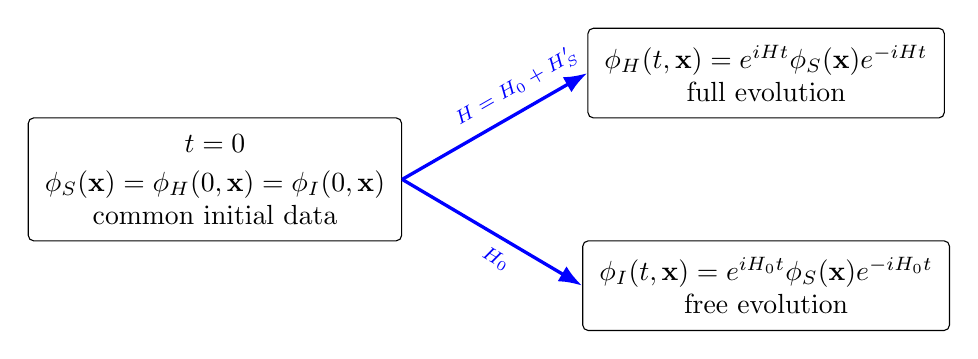
\begin{tikzpicture}[
  >=Latex,
  box/.style={draw,rounded corners=2pt,align=center,inner sep=6pt},
  evolution/.style={->,very thick,blue}
]
  \node[box] (initial) at (0,0)
    {$t=0$\\[2pt]
    $\phi_S(\mathbf{x})=\phi_H(0,\mathbf{x})=\phi_I(0,\mathbf{x})$\\
    common initial data};
  \node[box] (heis) at (7.0,1.35)
    {$\phi_H(t,\mathbf{x})=e^{iHt}\phi_S(\mathbf{x})e^{-iHt}$\\
    full evolution};
  \node[box] (inter) at (7.0,-1.35)
    {$\phi_I(t,\mathbf{x})=e^{iH_0t}\phi_S(\mathbf{x})e^{-iH_0t}$\\
    free evolution};
  \draw[evolution] (initial.east) --
    node[pos=0.68,above=3pt,sloped,fill=white,inner sep=1pt] {\scriptsize $H=H_0+H'_S$}
    (heis.west);
  \draw[evolution] (initial.east) --
    node[pos=0.58,below=3pt,sloped,fill=white,inner sep=1pt] {\scriptsize $H_0$}
    (inter.west);
\end{tikzpicture}
\diagramcaption{Summary of \eqref{eq:fieldHeisenberg} and \eqref{eq:fieldInteraction}:
the same initial data evolve with $H$ to give $\phi_H$ and with $H_0$ to give $\phi_I$.}
\end{minipage}
\end{center}

\subsection{States and operators in each picture}

\begin{definicion}[Schrödinger picture]
States evolve with the full Hamiltonian, while operators without
explicit time dependence remain fixed:
\begin{equation}
  \eqbox{\ket{\psi_S(t)}\coloneqq e^{-iHt}\ket{\psi_S(0)},
  \qquad \frac{\partial A_S}{\partial t}=0.}
\end{equation}
Therefore, the operator is denoted by $A_S$, without a time argument; it is not written as $A_S(t)$.
\end{definicion}

\begin{definicion}[Heisenberg picture]
States are constant and operators evolve with the full Hamiltonian:
\begin{equation}
  \eqbox{\ket{\psi_H}\coloneqq\ket{\psi_S(0)},
  \qquad
  A_H(t)\coloneqq e^{iHt}A_Se^{-iHt}.}
\end{equation}
\end{definicion}

\begin{definicion}[Interaction picture]
Operators evolve with $H_0$:
\begin{equation}
  \eqbox{A_I(t)
  \coloneqq e^{iH_0t}A_Se^{-iH_0t}.}
  \label{eq:AI}
\end{equation}

From the definition of the Heisenberg picture,
\begin{equation}
  A_H(t)=e^{iHt}A_Se^{-iHt},
\end{equation}
we solve for
\begin{equation}
  A_S=e^{-iHt}A_H(t)e^{iHt}.
\end{equation}
Substituting this result into \eqref{eq:AI},
\begin{equation}
  \eqbox{A_I(t)
  =e^{iH_0t}e^{-iHt}A_H(t)e^{iHt}e^{-iH_0t}.}
  \label{eq:AIfromAHexplicit}
\end{equation}
\begin{equation}
  \eqbox{A_I(t)=U_I(t)A_H(t)U_I^\dagger(t).}
  \label{eq:AIfromAH}
\end{equation}
where
\begin{equation}
  \eqbox{U_I(t)\coloneqq e^{iH_0t}e^{-iHt}.}
  \label{eq:UI}
\end{equation}
Applied to the field, relation \eqref{eq:AIfromAHexplicit} shows that the
transformation to the interaction picture cancels the full evolution,
leaving only free evolution:
\begin{align}
  \phi_I(t,\mathbf{x})
  &=e^{iH_0t}e^{-iHt}\phi_H(t,\mathbf{x})e^{iHt}e^{-iH_0t}
  \notag\\
  &=e^{iH_0t}e^{-iHt}
    \left(e^{iHt}\phi_S(\mathbf{x})e^{-iHt}\right)
    e^{iHt}e^{-iH_0t}
  \notag\\
  &=e^{iH_0t}\phi_S(\mathbf{x})e^{-iH_0t}.
  \label{eq:phiIfromphiH}
\end{align}
Equivalently,
\begin{equation}
  \eqbox{A_H(t)=U_I^\dagger(t)A_I(t)U_I(t).}
\end{equation}

States carry the remaining evolution:
\begin{equation}
  \ket{\psi_I(t)}\coloneqq e^{iH_0t}\ket{\psi_S(t)},
  \qquad
  i\frac{d}{dt}\ket{\psi_I(t)}=H'_I(t)\ket{\psi_I(t)},
\end{equation}
\end{definicion}



\begin{center}
\begin{minipage}{\linewidth}
\centering
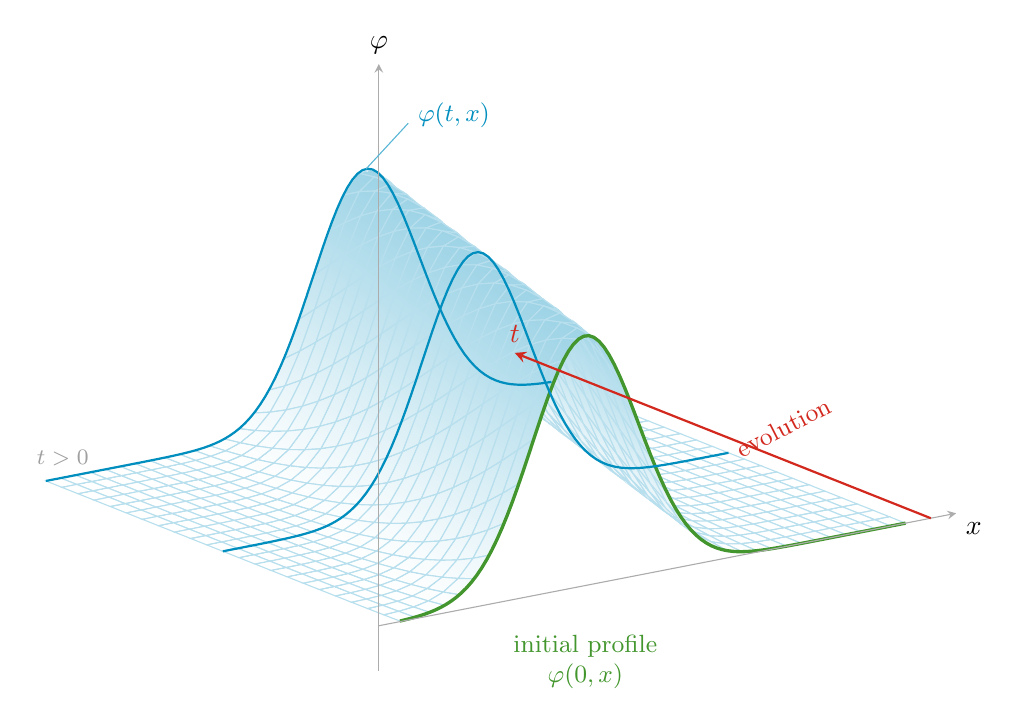
\begin{tikzpicture}
\begin{axis}[
 width=12.5cm,height=8.9cm,view={-35}{27},
 axis lines=none,ticks=none,
 xmin=-3,xmax=3,ymin=0,ymax=4,zmin=0,zmax=1.35,
 clip=false,z buffer=sort,
 colormap={campo}{color(0cm)=(white);color(1cm)=(diagramblue!38!white)}]
% x is position, y is time, and z is the value of an illustrative profile.
\addplot3[surf,shader=faceted interp,faceted color=diagramblue!28,
 domain=-3:3,y domain=0:4,samples=35,samples y=23]
 {exp(-1.25*(x-.4*y+.8)^2)};
% The initial profile is highlighted and forms the edge of the surface.
\addplot3[diagramgreen,very thick,domain=-3:3,samples=100,samples y=1]
 (x,0,{exp(-1.25*(x+.8)^2)});
% Two later profiles show spatial slices of the evolution.
\addplot3[diagramblue,thick,domain=-3:3,samples=100,samples y=1]
 (x,2,{exp(-1.25*x^2)});
\addplot3[diagramblue,thick,domain=-3:3,samples=100,samples y=1]
 (x,4,{exp(-1.25*(x-.8)^2)});
% The three axes have distinct meanings.
\draw[gray!65,->,>=stealth,thin] (axis cs:-3.25,0,0)--(axis cs:3.6,0,0)
 node[below right,text=black] {$x$};
\draw[diagramred,->,>=stealth,thick] (axis cs:3.3,0,0)--(axis cs:3.3,4.7,0)
 node[above,text=diagramred] {$t$};
\draw[gray!65,->,>=stealth,thin] (axis cs:-3.25,0,-.18)--(axis cs:-3.25,0,2.25)
 node[above,text=black] {$\varphi$};
\node[anchor=north,text=diagramgreen,font=\small,align=center]
 at (axis cs:-.8,0,-.16) {initial profile\\$\varphi(0,x)$};
\node[anchor=west,text=diagramblue,font=\small]
 at (axis cs:1.3,4,1.18) {$\varphi(t,x)$};
\draw[diagramblue!65,thin] (axis cs:1.3,4,1.15)--(axis cs:.8,4,1);
\node[text=diagramred,font=\small,rotate=27]
 at (axis cs:3.65,2,.06) {evolution};
\node[text=gray!75,font=\footnotesize]
 at (axis cs:-2.8,4,.08) {$t>0$};
\end{axis}
\end{tikzpicture}
\diagramcaption{From the spatial profile to its time evolution. The green curve
represents an initial profile at $t=0$; the blue slices show later profiles.
The red axis indicates time, and height indicates the value of the field.
The surface is a schematic classical profile, not a graph of the quantum
operator or a computed solution of $\lambda\phi^4$ theory.}
\end{minipage}
\end{center}

The figure illustrates how a spatial profile extends through time.
In the operator definitions, the same time appears in both $\phi_I$ and
$\phi_H$; their evolutions differ through the generator, $H_0$ or $H$.

A concrete example in one spatial dimension is the free mode
\[
 \varphi(t,x)=A\cos(kx-\omega_k t),\qquad
 \omega_k=\sqrt{k^2+m^2}.
\]
At $t=0$ we have the profile $A\cos(kx)$; at later times,
the phase $-\omega_k t$ shifts the crests and troughs. This wave is an
analytical example of free evolution; the surface in the drawing merely
illustrates the geometric construction of a profile over time.

\section{Interaction Hamiltonian}

To express $H'_I(t)$ in terms of free fields, we first verify,
using the mode expansion, the evolution with $H_0$ defined in
\eqref{eq:fieldInteraction}.

\subsection{Reconstructing the free field}

\begin{ejemplo}[Verification of free evolution]
We write the common initial operator $\phi_S(\mathbf{x})=\phi_I(0,\mathbf{x})$
in the mode expansion associated with the free Hamiltonian $H_0$:
\begin{equation}
  \phi_S(\mathbf{x})=
  \int\frac{d^3k}{(2\pi)^3}\frac{1}{\sqrt{2\omega_{\mathbf{k}}}}
  \left[
    a_{\mathbf{k}}e^{i\mathbf{k}\cdot\mathbf{x}}
    +a_{\mathbf{k}}^\dagger e^{-i\mathbf{k}\cdot\mathbf{x}}
  \right].
  \label{eq:freefield0}
\end{equation}
Here $\omega_{\mathbf{k}}\coloneqq\sqrt{\mathbf{k}^2+m^2}$.
The operators $a_{\mathbf{k}}$ and $a_{\mathbf{k}}^\dagger$ are defined
with respect to this free part, whose vacuum satisfies $a_{\mathbf{k}}\ket{0}=0$.
Consider the free Hamiltonian, omitting the zero-point energy constant,
\begin{equation}
  H_0=\int\frac{d^3k}{(2\pi)^3}\,
  \omega_{\mathbf{k}}a_{\mathbf{k}}^\dagger a_{\mathbf{k}},
\end{equation}
and the commutation relations
\begin{equation}
  [a_{\mathbf{k}},a_{\mathbf{p}}^\dagger]
  =(2\pi)^3\delta^{(3)}(\mathbf{k}-\mathbf{p}),
  \qquad
  [a_{\mathbf{k}},a_{\mathbf{p}}]
  =[a_{\mathbf{k}}^\dagger,a_{\mathbf{p}}^\dagger]=0.
\end{equation}
Show, using nested commutators and the Baker--Campbell--Hausdorff
formula, that
\begin{equation}
  \boxed{\begin{aligned}
  e^{iH_0t}\phi_S(\mathbf{x})e^{-iH_0t}
  &={}\int\frac{d^3k}{(2\pi)^3}\frac{1}{\sqrt{2\omega_{\mathbf{k}}}}
  \left[
    a_{\mathbf{k}}e^{-i\omega_{\mathbf{k}}t+i\mathbf{k}\cdot\mathbf{x}}
    +a_{\mathbf{k}}^\dagger e^{i\omega_{\mathbf{k}}t-i\mathbf{k}\cdot\mathbf{x}}
  \right].
  \end{aligned}}
  \label{eq:freefield}
\end{equation}
Conclude that the evolution generated by $H_0$ reconstructs the free
Klein--Gordon field $\phi_{\mathrm{libre}}(t,\mathbf{x})$.

\par\smallskip\noindent\textbf{Solution.}
According to the definition of the interaction picture, we compute
\begin{equation}
  \eqbox{\phi_I(t,\mathbf{x})
  =e^{iH_0t}\phi_S(\mathbf{x})e^{-iH_0t}.}
  \label{eq:fieldBCH}
\end{equation}
We first obtain the elementary commutators\footnote{We use
\([AB,C]=A[B,C]+[A,C]B\). Entonces
\begin{align*}
[H_0,a_{\mathbf{k}}]
&=\int\frac{d^3p}{(2\pi)^3}\,
\omega_{\mathbf{p}}
[a_{\mathbf{p}}^\dagger a_{\mathbf{p}},a_{\mathbf{k}}] \\
&=\int\frac{d^3p}{(2\pi)^3}\,
\omega_{\mathbf{p}}
\bigl(a_{\mathbf{p}}^\dagger[a_{\mathbf{p}},a_{\mathbf{k}}]
+[a_{\mathbf{p}}^\dagger,a_{\mathbf{k}}]a_{\mathbf{p}}\bigr) \\
&=-\int\frac{d^3p}{(2\pi)^3}\,
\omega_{\mathbf{p}}(2\pi)^3
\delta^{(3)}(\mathbf{p}-\mathbf{k})a_{\mathbf{p}}
=-\omega_{\mathbf{k}}a_{\mathbf{k}}.
\fnEqTag
\end{align*}
and similarly
\begin{align*}
[H_0,a_{\mathbf{k}}^\dagger]
&=\int\frac{d^3p}{(2\pi)^3}\,
\omega_{\mathbf{p}}
[a_{\mathbf{p}}^\dagger a_{\mathbf{p}},a_{\mathbf{k}}^\dagger] \\
&=\int\frac{d^3p}{(2\pi)^3}\,
\omega_{\mathbf{p}}
a_{\mathbf{p}}^\dagger[a_{\mathbf{p}},a_{\mathbf{k}}^\dagger]
=\omega_{\mathbf{k}}a_{\mathbf{k}}^\dagger .
\fnEqTag
\end{align*}
}
\begin{equation}
  [H_0,a_{\mathbf{k}}]=-\omega_{\mathbf{k}}a_{\mathbf{k}},
  \qquad
  [H_0,a_{\mathbf{k}}^\dagger]=\omega_{\mathbf{k}}a_{\mathbf{k}}^\dagger.
  \label{eq:H0akcomm}
\end{equation}

We now apply the Baker--Campbell--Hausdorff conjugation formula
(also called Hadamard's lemma) with
$A=iH_0t$ and $B=\phi_S(\mathbf{x})=\phi_I(0,\mathbf{x})$:
\begin{equation}
  \boxed{\begin{gathered}\textstyle
  e^{iH_0t}B e^{-iH_0t}
  =
  B+it[H_0,B]
  +\frac{(it)^2}{2!}[H_0,[H_0,B]]
  +\frac{(it)^3}{3!}[H_0,[H_0,[H_0,B]]]+\cdots .
  \end{gathered}}
  \label{eq:BCHfield}
\end{equation}
Let us now compute the commutators appearing in \eqref{eq:BCHfield}.
Using \eqref{eq:H0akcomm} in expansion \eqref{eq:freefield0}, the first
commutator is
\begin{equation}
  [H_0,\phi_S(\mathbf{x})]
  =
  \int\frac{d^3k}{(2\pi)^3}
  \frac{1}{\sqrt{2\omega_{\mathbf{k}}}}
  \left[
    -\omega_{\mathbf{k}}a_{\mathbf{k}}e^{i\mathbf{k}\cdot\mathbf{x}}
    +\omega_{\mathbf{k}}a_{\mathbf{k}}^\dagger e^{-i\mathbf{k}\cdot\mathbf{x}}
  \right].
  \label{eq:firstPhiComm}
\end{equation}
Commuting once more with \(H_0\),
\begin{equation}
  [H_0,[H_0,\phi_S(\mathbf{x})]]
  =
  \int\frac{d^3k}{(2\pi)^3}
  \frac{1}{\sqrt{2\omega_{\mathbf{k}}}}
  \left[
    \omega_{\mathbf{k}}^2a_{\mathbf{k}}e^{i\mathbf{k}\cdot\mathbf{x}}
    +\omega_{\mathbf{k}}^2a_{\mathbf{k}}^\dagger e^{-i\mathbf{k}\cdot\mathbf{x}}
  \right].
  \label{eq:secondPhiComm}
\end{equation}
The third commutator already reveals the alternating signs:
\begin{equation}
  [H_0,[H_0,[H_0,\phi_S(\mathbf{x})]]]
  =
  \int\frac{d^3k}{(2\pi)^3}
  \frac{1}{\sqrt{2\omega_{\mathbf{k}}}}
  \left[
    -\omega_{\mathbf{k}}^3a_{\mathbf{k}}e^{i\mathbf{k}\cdot\mathbf{x}}
    +\omega_{\mathbf{k}}^3a_{\mathbf{k}}^\dagger e^{-i\mathbf{k}\cdot\mathbf{x}}
  \right].
  \label{eq:thirdPhiComm}
\end{equation}
Thus, for \(n\) nested commutators,
\begin{equation}
  \underbrace{[H_0,[H_0,\cdots[H_0,\phi_S(\mathbf{x})]\cdots]]}_{n\ \text{times}}
  =
  \int\frac{d^3k}{(2\pi)^3}
  \frac{1}{\sqrt{2\omega_{\mathbf{k}}}}
  \left[
    (-\omega_{\mathbf{k}})^n
    a_{\mathbf{k}}e^{i\mathbf{k}\cdot\mathbf{x}}
    +\omega_{\mathbf{k}}^n
    a_{\mathbf{k}}^\dagger e^{-i\mathbf{k}\cdot\mathbf{x}}
  \right].
  \label{eq:nestedPhiComm}
\end{equation}
Substituting these commutators into \eqref{eq:BCHfield},
\begin{align}
  \phi_I(t,\mathbf{x})
  &\coloneqq e^{iH_0t}\phi_S(\mathbf{x})e^{-iH_0t}
  \notag\\
  &=
  \int\frac{d^3k}{(2\pi)^3}
  \frac{1}{\sqrt{2\omega_{\mathbf{k}}}}
  \left[
    a_{\mathbf{k}}e^{i\mathbf{k}\cdot\mathbf{x}}
    \sum_{n=0}^{\infty}\frac{(-i\omega_{\mathbf{k}}t)^n}{n!}
    +
    a_{\mathbf{k}}^\dagger e^{-i\mathbf{k}\cdot\mathbf{x}}
    \sum_{n=0}^{\infty}\frac{(i\omega_{\mathbf{k}}t)^n}{n!}
  \right]
  \notag\\
  &=
  \int\frac{d^3k}{(2\pi)^3}
  \frac{1}{\sqrt{2\omega_{\mathbf{k}}}}
  \left[
    a_{\mathbf{k}}e^{-i\omega_{\mathbf{k}}t+i\mathbf{k}\cdot\mathbf{x}}
    +
    a_{\mathbf{k}}^\dagger
    e^{i\omega_{\mathbf{k}}t-i\mathbf{k}\cdot\mathbf{x}}
  \right]
  \equiv\phi_{\mathrm{libre}}(t,\mathbf{x}).
  \label{eq:BCHsubstitutionField}
\end{align}
The last equality defines the notation $\phi_{\mathrm{libre}}(t,\mathbf{x})$
for the free Klein--Gordon field given by this mode expansion. Therefore,
\begin{equation}
  \eqbox{\phi_I(t,\mathbf{x})=\phi_{\mathrm{libre}}(t,\mathbf{x}).}
  \label{eq:BCHrecoversField}
\end{equation}
Summing the commutators reconstructs the phases $e^{\mp i\omega_{\mathbf{k}}t}$
and verifies the mode expansion of the free field stated in the problem.
\end{ejemplo}

\begin{observacion}
The field $\phi_I$ is not a ``part'' of $\phi_H$ in an additive sense.
It is the free field with which we organize the effect of $H'_I(t)$
perturbatively.
\end{observacion}

\subsection{Constructing the interaction}

Having computed the field $\phi_I$, we transform a different operator:
the interaction term $H'_S$ defined in \eqref{eq:Hprime}. Recall that
\begin{equation}
  H'_S=\frac{\lambda}{4!}\int d^3z\,\phi_S^4(\mathbf{z}).
\end{equation}
Its expression in the interaction picture is
\begin{equation}
  \eqbox{H'_I(t)\coloneqq e^{iH_0t}H'_Se^{-iH_0t}.}
  \label{eq:HIdefinition}
\end{equation}
We now use the result of Example 1, \eqref{eq:BCHrecoversField}:
$e^{iH_0t}\phi_S(\mathbf{z})e^{-iH_0t}=\phi_I(t,\mathbf{z})$.
Conjugation preserves products: we insert $e^{-iH_0t}e^{iH_0t}=1$
between the four factors of $\phi_S^4$ and apply this result to each
factor. Substituting \eqref{eq:Hprime},
\begin{align}
  e^{iH_0t}H'_Se^{-iH_0t}
  &=\frac{\lambda}{4!}\int d^3z\,
    e^{iH_0t}\phi_S^4(\mathbf{z})e^{-iH_0t}
    \notag\\
  &=\frac{\lambda}{4!}\int d^3z\,
    \left(e^{iH_0t}\phi_S(\mathbf{z})e^{-iH_0t}\right)^4
    \notag\\
  &=\frac{\lambda}{4!}\int d^3z\,\phi_I^4(t,\mathbf{z}).
  \label{eq:HSaHI}
\end{align}
Therefore,
\begin{equation}
  \eqbox{H'_I(t)
  =e^{iH_0t}H'_Se^{-iH_0t}
  =\frac{\lambda}{4!}\int d^3z\,\phi_I^4(t,\mathbf{z}).}
  \label{eq:HIphi4}
\end{equation}

Only the interaction term appears here because we start from $H'_S$.
When transforming the total Hamiltonian, the free part is also present:
\begin{equation}
  e^{iH_0t}He^{-iH_0t}=H_0+H'_I(t).
  \label{eq:totalHamiltonianI}
\end{equation}
For states, however, the change of picture absorbs the free evolution.
Differentiating\newline
$\ket{\psi_I(t)}=e^{iH_0t}\ket{\psi_S(t)}$\allowbreak{} gives
\begin{align}
  i\frac{d}{dt}\ket{\psi_I(t)}
  &=\left[-H_0+e^{iH_0t}He^{-iH_0t}\right]\ket{\psi_I(t)}
  \notag\\
  &=H'_I(t)\ket{\psi_I(t)}.
  \label{eq:interactionGenerator}
\end{align}
The term $-H_0$ comes from differentiating $e^{iH_0t}$ and cancels
the free part of \eqref{eq:totalHamiltonianI}. This is why the Dyson
series, which describes the evolution of these states, uses $H'_I(t)$.

The interaction is used without normal ordering: the term $\phi_I^4$
is not replaced by $:\!\phi_I^4\!:$, so the local contractions that
give rise to the loops in the examples are retained.

The integral in \eqref{eq:HIphi4} runs over all space at a fixed time.
Therefore, $H'_I(t)$ still depends on $t$. Time is subsequently integrated
in the Dyson series:
\begin{equation}
  \eqbox{\int_{-\infty}^{\infty}dt\,H'_I(t)
  =\frac{\lambda}{4!}\int d^4z\,\phi_I^4(z),
  \qquad z\coloneqq(t,\mathbf{z}).}
  \label{eq:intHI}
\end{equation}

\section{Starting point of the perturbative calculation}

Having constructed $\phi_I$ and $H'_I$, our calculations begin with the
Gell-Mann--Low formula\footnote{Murray Gell-Mann and Francis E. Low
introduced this result in the context of the perturbative formulation
of quantum field theories. In these notes, we use it as the rule that
allows expectation values in the interacting vacuum $\ket{\Omega}$ to be
written as ratios of expectation values in the free vacuum $\ket{0}$.}
for the two-point correlator.
Indeed, this formula works precisely because it replaces correlators of
the full field with correlators of the free Klein--Gordon field, together
with the time-ordered insertion of the interaction.
\begin{equation}
  \boxed{\displaystyle
  \mel{\Omega}{T\{\phi(x)\phi(y)\}}{\Omega}
  =
  \frac{
    \mel{0}{T\{\phi_I(x)\phi_I(y)
    e^{-i\int_{-\infty}^{\infty}dt\,H'_I(t)}\}}{0}
  }{
    \mel{0}{T\{e^{-i\int_{-\infty}^{\infty}dt\,H'_I(t)}\}}{0}
  }
  \coloneqq\frac{N}{D}.}
  \label{eq:GML}
\end{equation}
Here $\phi(x)$ denotes $\phi_H(x)$, the full field in the Heisenberg
picture; $\ket{\Omega}$ is the interacting vacuum and $\ket{0}$ the free
vacuum, both normalized. The symbols $N$ and $D$ denote the numerator
and denominator of \eqref{eq:GML}, respectively.
The formula is used perturbatively, with vacuum preparation and time
limits defined by a convergence prescription compatible with Feynman
conditions. The free vacuum is assumed to have nonzero overlap with
the interacting vacuum in the regularized theory. The $i\epsilon$ fixes
the pole prescription for propagators; it does not remove ultraviolet
divergences, which require regularization and renormalization.

Substituting \eqref{eq:HIphi4} into \eqref{eq:GML}, the evolution operator
contains, by \eqref{eq:intHI}, the exponential of
$-i\frac{\lambda}{4!}\int d^4z\,\phi_I^4(z)$ under time ordering.
We first expand the exponential formally in its Taylor series:
\begin{equation}
  \begin{aligned}
  \exp\left[-i\frac{\lambda}{4!}\int d^4z\,\phi_I^4(z)\right]
  &=1-i\frac{\lambda}{4!}\int d^4z\,\phi_I^4(z)
  \\
  &\quad+\frac{1}{2!}\left(-i\frac{\lambda}{4!}\right)^2
  \left[\int d^4z\,\phi_I^4(z)\right]^2+\cdots .
  \end{aligned}
  \label{eq:DysonTaylor}
\end{equation}
In the quadratic term, each integral factor has its own integration
variable. Since $z$ is a dummy variable, we may call them $z_1$ and $z_2$:
\begin{equation}
  \begin{aligned}
  \left[\int d^4z\,\phi_I^4(z)\right]^2
  &=\left[\int d^4z_1\,\phi_I^4(z_1)\right]
    \left[\int d^4z_2\,\phi_I^4(z_2)\right]
  \\
  &=\int d^4z_1\int d^4z_2\,
    \phi_I^4(z_1)\phi_I^4(z_2).
  \end{aligned}
  \label{eq:DysonIndependentVariables}
\end{equation}
The points $z_1$ and $z_2$ are integrated independently; squaring the
integral produces fields evaluated at both points, not eight fields at
a single point. At order $n$, there are $n$ variables $z_1,\ldots,z_n$,
one for each integral factor. We now apply $T$ to the fields in each
term, ordering them according to their times $z_j=(t_j,\mathbf{z}_j)$,
and obtain
\begin{equation}
  \boxed{\begin{aligned}
  T\left\{\exp\left[-i\frac{\lambda}{4!}
  \int d^4z\,\phi_I^4(z)\right]\right\}
  &=1-i\frac{\lambda}{4!}\int d^4z_1\,
  T\{\phi_I^4(z_1)\}
  \\
  &\quad
  +\frac{(-i\lambda)^2}{2!(4!)^2}
  \int d^4z_1\int d^4z_2\,
  T\{\phi_I^4(z_1)\phi_I^4(z_2)\}+\cdots .
  \end{aligned}}
  \label{eq:Dyson}
\end{equation}

Therefore,
\begin{align}
  N
  &=\mel{0}{T\{\phi_I(x)\phi_I(y)\}}{0}
  -i\frac{\lambda}{4!}\int d^4z\,
  \mel{0}{T\{\phi_I(x)\phi_I(y)\phi_I^4(z)\}}{0}
  +O(\lambda^2),\\
  D
  &=1-i\frac{\lambda}{4!}\int d^4z\,
  \mel{0}{T\{\phi_I^4(z)\}}{0}
  +O(\lambda^2).
\end{align}
The denominator $D$ contains the vacuum bubbles. When forming the ratio
$N/D$, these disconnected pieces cancel, ultimately leaving the
contributions connected to the external pair $x,y$.

\section{Wick's theorem at first order}

The basic contraction is the free propagator
\begin{equation}
  \Delta_F(a-b)
  \coloneqq\mel{0}{T\{\phi_I(a)\phi_I(b)\}}{0}.
\end{equation}
The contractions of the six-field term are grouped as
\begin{equation}
  \boxed{\begin{aligned}
  \mel{0}{T\{\phi_I(x)\phi_I(y)\phi_I^4(z)\}}{0}
  &=3\,\Delta_F(x-y)\bigl[\Delta_F(z-z)\bigr]^2
  \\
  &\quad
  +12\,\Delta_F(x-z)\Delta_F(y-z)\Delta_F(z-z).
  \end{aligned}}
  \label{eq:Wick6}
\end{equation}
The factor $3$ corresponds to contractions in which $x$ is joined to $y$;
the factor $12$ corresponds to contractions in which both external
points are joined to the vertex.

For the denominator, Wick's theorem allows the four fields at $z$ to
be paired in three ways. If we temporarily label the fields $1,2,3,4$,
the pairings are $(12)(34)$, $(13)(24)$, and $(14)(23)$. They all give
the same product of two propagators:
\begin{equation}
  \mel{0}{T\{\phi_I^4(z)\}}{0}
  =3\bigl[\Delta_F(z-z)\bigr]^2,
  \qquad \frac{3}{4!}=\frac{1}{8}.
  \label{eq:WickVacuumFour}
\end{equation}
From \eqref{eq:Wick6} and \eqref{eq:WickVacuumFour},
\begin{align}
  N
  &=\Delta_F(x-y)
  -i\lambda\int d^4z\left[
    \frac{1}{8}\Delta_F(x-y)\bigl[\Delta_F(z-z)\bigr]^2
  \right.
  \notag\\
  &\hspace{5.4cm}\left.
    +\frac{1}{2}\Delta_F(x-z)\Delta_F(y-z)\Delta_F(z-z)
  \right]+O(\lambda^2),\\
  D
  &=1-i\frac{\lambda}{8}\int d^4z\,
  \bigl[\Delta_F(z-z)\bigr]^2+O(\lambda^2).
\end{align}

\begin{center}
\begin{minipage}{\linewidth}
\centering
  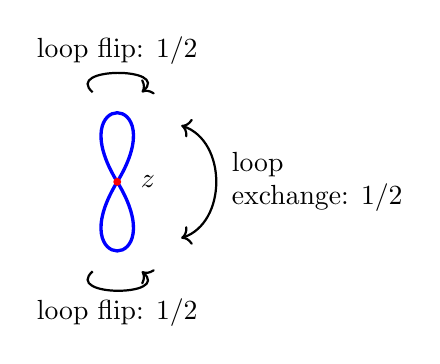
\begin{tikzpicture}[scale=0.65,baseline=(current bounding box.center)]
    \draw[blue,very thick] (0,0)
      .. controls (-1.1,1.8) and (1.1,1.8) .. (0,0);
    \draw[blue,very thick] (0,0)
      .. controls (-1.1,-1.8) and (1.1,-1.8) .. (0,0);
    \fill[red] (0,0) circle (2.2pt);
    \node[right=5pt,text=black] at (0,0) {$z$};
    \draw[->,thick] (-0.48,1.75)
      .. controls (-1.05,2.25) and (1.05,2.25) .. (0.48,1.75);
    \node[above] at (0,2.1) {loop flip: $1/2$};
    \draw[->,thick] (-0.48,-1.75)
      .. controls (-1.05,-2.25) and (1.05,-2.25) .. (0.48,-1.75);
    \node[below] at (0,-2.1) {loop flip: $1/2$};
    \draw[<->,thick] (1.25,1.1)
      .. controls (2.15,0.8) and (2.15,-0.8) .. (1.25,-1.1);
    \node[right,align=left] at (2.05,0)
      {loop\\exchange: $1/2$};
  \end{tikzpicture}
  \diagramcaption{Figure-eight vacuum bubble: two loops joined at a vertex.}
\end{minipage}
\end{center}
Its symmetry factor is $S=2\cdot2\cdot2=8$\footnote{See K.~Peeters and
M.~Zamaklar, \textit{A guide to quantum field theory}, Section 4.3,
the discussion of equation (4.34), pp.~31--32: the flips of each loop
and the exchange of the two loops of the figure eight are counted.
\href{https://maths.dur.ac.uk/users/kasper.peeters/pdf/qft2.pdf}{Durham notes}.}:
we can exchange the two ends of each loop and also exchange the loops
with each other without changing the diagram. Each of these symmetries
of order two contributes a factor $1/2$:
\begin{equation}
  \frac{1}{S}=\frac{1}{2}\,\frac{1}{2}\,\frac{1}{2}=\frac{1}{8},
  \qquad
  \mathcal{A}_{\mathrm{vac}}^{(1)}
  =\frac{-i\lambda}{8}\int d^4z\,\bigl[\Delta_F(z-z)\bigr]^2.
\end{equation}
Exchanging the ends of a loop is often visualized as a flip of the loop;
what is counted is that discrete permutation, not an arbitrary rotation
of the drawing. This is a single vacuum bubble with two loops, not two
independent bubbles. The $1/8$ obtained from Wick's theorem already
includes these symmetries: one does not divide by $8$ again.

\subsection{Cancellation of vacuum bubbles}
Cancellation does not occur only at first order. Each diagram in the
numerator separates into a part attached to the external points $x,y$
and a collection of vacuum bubbles disconnected from them. These
bubbles form exactly the same factor that appears in the denominator.
Diagrammatically, the normalization is written as

\begin{equation}
  \boxed{\begin{aligned}
  \frac{N}{D}
  &=\frac{
    \left[\qftFreeDiagram+\qftTadpoleDiagram+\qftChainDiagram+\cdots\right]
    \exp\left(\qftVacuumDiagram+\cdots\right)
  }{\exp\left(\qftVacuumDiagram+\cdots\right)}
  \\[0.8em]
  &=\qftFreeDiagram+\qftTadpoleDiagram+\qftChainDiagram+\cdots .
  \end{aligned}}
  \label{eq:VacuumDiagramCancellation}
\end{equation}
\begin{center}
\begin{minipage}{\linewidth}
\centering
  \diagramcaption{Cancellation of vacuum bubbles in the normalized correlator.}
\end{minipage}
\end{center}

Each drawing represents its full contribution, with the corresponding
propagators, vertices, integrals, and symmetry factors. The endpoints
of the open lines are $x,y$. The exponential contains the sum of
connected vacuum bubbles; expanding it also generates collections of
independent bubbles, with their factors $1/n!$.

After canceling the common vacuum-bubble factor in
\eqref{eq:VacuumDiagramCancellation}, the sum of diagrams connected to
the external pair $x,y$ remains. We assume a vacuum that preserves the
symmetry $\phi\mapsto-\phi$, so one-field correlators vanish. Loops
attached to the external points, such as the \emph{tadpole} loop,
remain in this sum.

To obtain the correlator through first order, we retain only the first
two diagrams: free propagation, of order $\lambda^0$, and the
\emph{tadpole}, of order $\lambda$. The chain and all other terms of
second or higher order are included in $O(\lambda^2)$:
\begin{equation}
  \eqbox{\frac{N}{D}
  =\qftFreeDiagram+\qftTadpoleDiagram+O(\lambda^2).}
  \label{eq:VacuumFactorCancellation}
\end{equation}
Writing the contributions of these two diagrams in position space gives
 directly
\begin{equation}
  \eqbox{\mel{\Omega}{T\{\phi(x)\phi(y)\}}{\Omega}
  =\Delta_F(x-y)
  -i\frac{\lambda}{2}\int d^4z\,
  \Delta_F(x-z)\Delta_F(y-z)\Delta_F(z-z)
  +O(\lambda^2).}
  \label{eq:G2primerorden}
\end{equation}
The zeroth-order term has $S=1$, and the first-order \emph{tadpole} has
$S=2$. The three second-order topologies are developed in the next section.
Here $\Delta_F(z-z)=\Delta_F(0)$ is formally ultraviolet divergent and
must be regularized and renormalized.\footnote{\begin{minipage}[t]{\dimexpr\linewidth-1.8em\relax}
With our convention,
\begin{equation*}
 \Delta_F(0)=\int\frac{d^3p}{(2\pi)^3}
 \frac{1}{2\sqrt{\mathbf p^2+m^2}}.
 \fnEqTag
\end{equation*}
At large momenta, the radial measure turns the integral into an
expression that grows as $\int p\,dp$: hence the ultraviolet divergence,
associated with short wavelengths.
A cutoff $|\mathbf p|\leq\Lambda$ regularizes the integral:
\begin{equation*}
 \Delta_F^{(\Lambda)}(0)=\frac{1}{4\pi^2}
 \int_0^\Lambda\frac{p^2\,dp}{\sqrt{p^2+m^2}}
 \sim\frac{\Lambda^2}{8\pi^2},\qquad \Lambda\gg m.
 \fnEqTag
\end{equation*}
Renormalization adjusts parameters and counterterms through physical
conditions to obtain finite predictions when the regulator is removed.
In this tadpole, the divergence is absorbed into the mass counterterm;
it is not a vacuum bubble that cancels, nor does it change $S=2$.
See Peeters and Zamaklar,
\href{https://maths.dur.ac.uk/users/kasper.peeters/pdf/qft2.pdf}
{\textit{A guide to quantum field theory}}, Sections 7.1 and 7.2.\end{minipage}}
The symmetry factors are unchanged.

\section{Connected contributions at second order}

For the interaction $\lambda\phi^4/4!$ without normal ordering, the
three connected topologies of the two-point correlator at second
order are as follows:

Two \emph{tadpole} diagrams (``tadpoles'') in a chain:

\begin{center}
\begin{minipage}{\linewidth}
\centering
  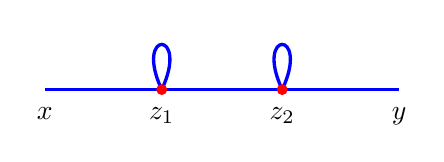
\begin{tikzpicture}[scale=0.9,baseline=(current bounding box.center)]
    \draw[blue,very thick] (-2.5,0)--(2.5,0);
    \draw[blue,very thick] (-0.85,0)
      .. controls (-1.25,0.85) and (-0.45,0.85) .. (-0.85,0);
    \draw[blue,very thick] (0.85,0)
      .. controls (0.45,0.85) and (1.25,0.85) .. (0.85,0);
    \fill[red] (-0.85,0) circle (2.2pt) node[below=3pt,text=black] {$z_1$};
    \fill[red] (0.85,0) circle (2.2pt) node[below=3pt,text=black] {$z_2$};
    \node[below=3pt] at (-2.5,0) {$x$};
    \node[below=3pt] at (2.5,0) {$y$};
  \end{tikzpicture}
  \diagramcaption{Two \emph{tadpole} diagrams in a chain.}
\end{minipage}
\end{center}
\begin{align}
  &\frac{(-i\lambda)^2}{4}
  \int d^4z_1\int d^4z_2\,
  \Delta_F(x-z_1)\Delta_F(z_1-z_1)
  \notag\\[-0.2em]
  &\hspace{3.2cm}\times
  \Delta_F(z_1-z_2)\Delta_F(z_2-z_2)\Delta_F(z_2-y).
  \label{eq:G2chainContribution}
\end{align}


Two lines between vertices and a local loop:
\begin{center}
\begin{minipage}{\linewidth}
\centering
  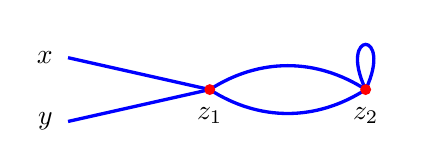
\begin{tikzpicture}[scale=0.9,baseline=(current bounding box.center)]
    \draw[blue,very thick] (-2.7,0.45)--(-0.7,0);
    \draw[blue,very thick] (-2.7,-0.45)--(-0.7,0);
    \draw[blue,very thick] (-0.7,0)
      .. controls (0.0,0.45) and (0.8,0.45) .. (1.5,0);
    \draw[blue,very thick] (-0.7,0)
      .. controls (0.0,-0.45) and (0.8,-0.45) .. (1.5,0);
    \draw[blue,very thick] (1.5,0)
      .. controls (1.1,0.85) and (1.9,0.85) .. (1.5,0);
    \fill[red] (-0.7,0) circle (2.2pt) node[below=3pt,text=black] {$z_1$};
    \fill[red] (1.5,0) circle (2.2pt) node[below=3pt,text=black] {$z_2$};
    \node[left=2pt] at (-2.7,0.45) {$x$};
    \node[left=2pt] at (-2.7,-0.45) {$y$};
  \end{tikzpicture}
  \diagramcaption{Two lines between vertices and a local loop.}
\end{minipage}
\end{center}
\begin{align}
  &\frac{(-i\lambda)^2}{4}
  \int d^4z_1\int d^4z_2\,
  \Delta_F(x-z_1)\Delta_F(y-z_1)
  \bigl[\Delta_F(z_1-z_2)\bigr]^2
  \Delta_F(z_2-z_2).
\end{align}

\emph{Sunset} diagram:
\begin{center}
\begin{minipage}{\linewidth}
\centering
  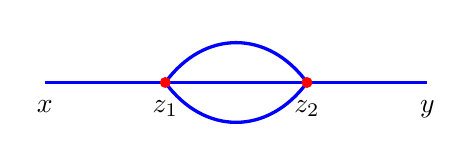
\begin{tikzpicture}[scale=0.9,baseline=(current bounding box.center)]
    \draw[blue,very thick] (-2.7,0)--(-1.0,0);
    \draw[blue,very thick] (1.0,0)--(2.7,0);
    \draw[blue,very thick] (-1.0,0)
      .. controls (-0.45,0.75) and (0.45,0.75) .. (1.0,0);
    \draw[blue,very thick] (-1.0,0)--(1.0,0);
    \draw[blue,very thick] (-1.0,0)
      .. controls (-0.45,-0.75) and (0.45,-0.75) .. (1.0,0);
    \fill[red] (-1.0,0) circle (2.2pt) node[below=3pt,text=black] {$z_1$};
    \fill[red] (1.0,0) circle (2.2pt) node[below=3pt,text=black] {$z_2$};
    \node[below=3pt] at (-2.7,0) {$x$};
    \node[below=3pt] at (2.7,0) {$y$};
  \end{tikzpicture}
  \diagramcaption{\emph{Sunset} diagram.}
\end{minipage}
\end{center}
\begin{equation}
  \frac{(-i\lambda)^2}{6}
  \int d^4z_1\int d^4z_2\,
  \Delta_F(x-z_1)
  \bigl[\Delta_F(z_1-z_2)\bigr]^3
  \Delta_F(z_2-y).
\end{equation}
The denominators $4$, $4$, and $6$ are the symmetry factors of these
topologies, respectively. They can also be obtained by counting the
contractions with the external points $x,y$ fixed: there are $288$,
$288$, and $192$ pairings, respectively. Dividing by the factor
$2!(4!)^2=1152$ from the Dyson expansion gives $1/4$, $1/4$, and $1/6$.

\section{Feynman rules in position space}

The preceding derivations give three rules for the interaction
$\lambda\phi^4/4!$:
\begin{enumerate}[label=\textbf{\arabic*.},leftmargin=1.8em,itemsep=0.7em]
  \item \textbf{Lines.} Each contraction between points $a$ and $b$
  contributes the propagator $\Delta_F(a-b)$, as in \qftFreeDiagram.
  \item \textbf{Vertices.} Each vertex has four line ends and contributes
  $(-i\lambda)\int d^4z$. Its position $z$ is integrated, while the external
  points $x,y$ stay fixed. With $V$ vertices there are $V$ independent
  integrations.
  \item \textbf{Symmetries.} Divide by the factor $S$, counting the
  permutations that preserve the diagram and fix the external points.
  For example, the \emph{tadpole} \qftTadpoleDiagram\ has $S=2$;
  the three second-order topologies have $S=4,4,6$.
\end{enumerate}

For a diagram with $V$ vertices, the three rules are summarized by
\begin{equation}
  \eqbox{\frac{1}{S}(-i\lambda)^V
  \int\prod_{j=1}^{V}d^4z_j
  \prod_{\text{lines }(ab)}\Delta_F(a-b).}
\end{equation}

To obtain the normalized correlator, sum the diagrams connected to the
external pair $x,y$ through the desired order, keeping those points fixed.
Vacuum bubbles have already canceled according to
\eqref{eq:VacuumDiagramCancellation}; loops attached to the external points
remain. The factor $1/S$ accounts for diagram symmetries and must not be
applied again when the coefficient has already been obtained by counting
Wick contractions.

\end{document}
